% Specification
% Gear Box for Machining Center
% P = 11kW
% n_output_max = 5000 min^{-1}

% Define a command to print variables as they get assigned.
% Use like \SetVar{variable_name}
% Command written by Heiko Oberdiek (http://tex.stackexchange.com/a/269392/45581) and edited by me.
\newcommand*{\SetVar}[2]{%
  \FPset{#1}{#2}
  \begingroup
    \fontencoding{T1}%
    \fontfamily{lmvtt}\selectfont % variable typewriter font
    % alternative: \ttfamily
    \detokenize{#1}% make _ to character
  \endgroup
  ~=~%
  \PrintVar{#1}
}
\newcommand*{\ExtractUnit}[1]{%
  \expandafter\ExtractUnitAux\detokenize{#1_}\relax
}
\begingroup
  \catcode`\_=12 %
  \gdef\ExtractUnitAux#1_#2\relax{%
    \ifx\\#2\\%
      #1
    \else
      \ExtractUnitAux#2\relax
    \fi
  }
\endgroup

% Command to print the value of a variable, together with the measurement unit.
% Written by me.
\newcommand*{\PrintVar}[1]
{
  \FPprint{#1}
  \,
  \ExtractUnit{#1}
}

% Command to multiply a variale by a floating point number.
\newcommand*{\Mul}[2]
{
  \FPeval{vTemp}{#1 * #2}
  \FPround\vTemp{\vTemp}{4}  % Round to four digits after decimal point.
  \FPprint{vTemp}
}

\documentclass{article}
\usepackage[nomessages]{fp}  % http://ctan.org/pkg/fp
\usepackage[pdftex]{graphicx}
\usepackage{gensymb}
\usepackage[T2A]{fontenc}
\usepackage[utf8]{inputenc}
\usepackage[bulgarian]{babel}
\usepackage[table]{xcolor}     % For coloured rows within tables.

\begin{document}

\begin{titlepage}
\begin{center}
\textsc{\Large Manufactoring Desing II Coursework}\\[1cm]
\textsc{\Huge Gearbox for Machining Center}\\[1.5cm]
\textsc{\Large Miroslav Vitkov}\\[0.5cm]
\textsc{Faculty number: 221207005}\\[1.5cm]
% TODO: include image of final design
\vfill
\today
\end{center}
\end{titlepage}

\section{Requirements}
Design a 2-speed gearbox for a vertical machining center.
The speeds needn't be changed at running motor. \\
\SetVar{P_output_kW}{11}          \\
\SetVar{P_output_max_rpm}{5000}

\section{Motor selection}
From [4] we select the Siemens 1PH209 spindle motor.
It is the recommended built-in motor for standard machine tool spindle.
Outside diameter is 205 mm, output shaft diameter 67 mm.
Nominal speed 1500 rpm, maximum 10000 rpm.
As the motor can be requested in different power ratings, we purchase one for 12kW as to compensate frcition losses.
\\
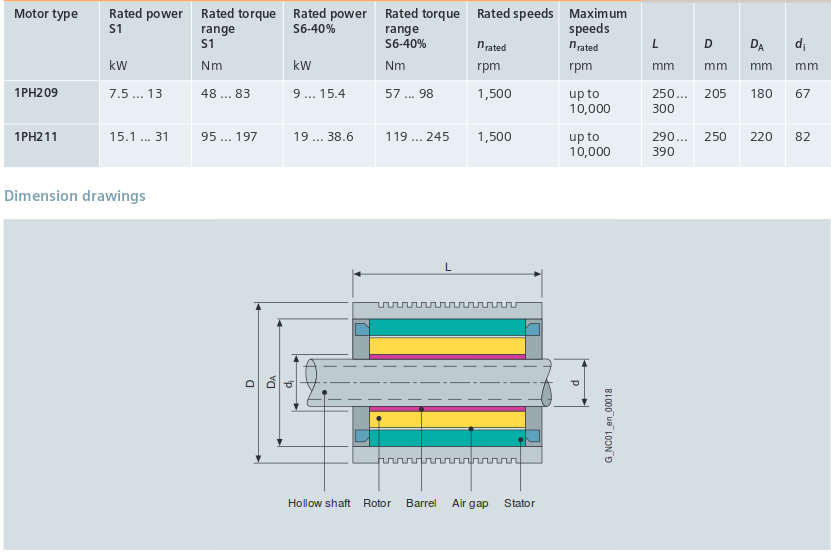
\includegraphics[width=1.25\textwidth]{images/motor}~

\section{Kinematic diagram} % (plan for rotational velocities)
The goal of the gearbox is to provide sufficient torque to the spindle at low motor speeds (below $n_{nominal}$).
For selecting the low gear we utilize the rule of thumb to choose a transfer ratio between $1/3$ and $1/4$:
$$ TR_{low} = 1/4 $$
For selecting the high gear, we try to match the maximum speed of the motor with the required maximum spindle speed by specification:
$$ TR_{high} = n_{spindle, max} / n_{motor, max} = 5000 / 10000 = 1/2$$
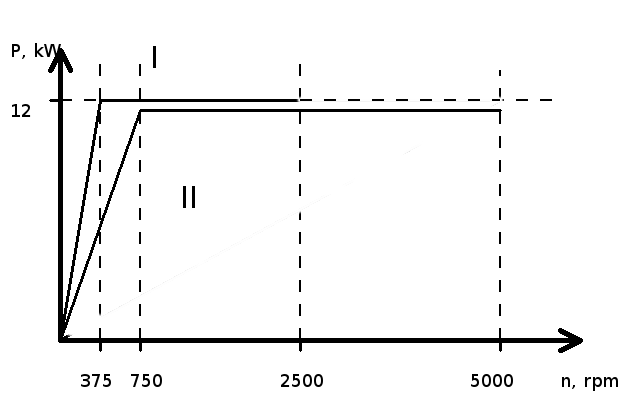
\includegraphics[width=0.75\textwidth]{images/kinematics}~

\section{Components sizing}
\subsection{Gears}
Requirements: Design input shaft gears G11 and G12 and output shaft gears G21 and G22
Both center distances (G11-G21 and G12-G22) must be equal.
All gears must be capable of transmitting the rated torque \PrintVar{P_output_kW} plus efficiency losses.
Gear teeth must be shaped with a cutoff or round-off to assist gear engagement.  % зъбозаобляне
Conventional spur gears with involute teeth profile have been selected for this application.
\subsubsection{Standard Basic Rack Tooth Profile}
Due to the numerous advantages of using standard tooth geometry, we decide to adhare to the Standard Basic Rack Tooth Profile [5]. \\
Pressure angle: $\alpha = 20\degree$  \\
Addendum circle: $h_a = 1.00m$ \\
Bottom clearance: $c = 0.25m$ \\
Daedendum circle: $h_f = 1.25m$ \\
Fillet radius: $\rho = 0.38m$ \\
Active tooth depth: $h_w = 2.00m$ \\
Whole depth: $h = 2.25m$ \\
Tooth thickness: $s = (\pi m)/ 2$ \\
\\
From [6] we select standard modules and number of teeth for G11, G12, G21 and G22.
We select arbitrary modules for the input gears and arbitrary number of teeth, limited by $z_{min} = 17$ and $z_{max} = 33$ [6].  \\
\FPset{vAlpha}{20\degree}
\FPset{TR_1_}{0.25}
\FPset{TR_2_}{0.5}
\SetVar{m_11_mm}{6} \\
\SetVar{m_12_mm}{6} \\
\SetVar{z_11_}{17} \\
\SetVar{z_12_}{20} \\ [0.5cm]
Now calculate the output gears.
For a transfer ratio of \PrintVar{TR_1_}, we would need G21 to have number of teeth: \\
\SetVar{z_21_}{\Mul{z_11_}{TR_1_}}  \\ % DIV!!!
\SetVar{m_21_mm}{6} \\
This results in a center distance for G11-G21 of: \\
\FPeval\vCenterDistance{m_11_mm * z_11_}
$$D_{base, G11} = \FPprint{vCenterDistance}$$
For a transfer ratio of \PrintVar{TR_2_}, we would need G22 to have number of teeth: \\
\SetVar{z_22_}{\Mul{z_12_}{TR_2_}}  \\  % DIV!!!
\SetVar{m_22_mm}{6} \\ [0.5cm]
The table below represents numerically the resulting geometry from module and teeth number choices. \\ [0.5cm]
\rowcolors{1}{white}{lightgray}
\begin{tabular}{l | c | c | c | c | c | c | c | c}
Gear & $\alpha$ & $h_a$, [mm]         & c, [mm]              & $h_f$, [mm]         & $\rho$, [mm]        & $h_w$, [mm]         & h, [mm]             & s, [mm] \\
G11  & \vAlpha  & \Mul{m_11_mm}{1.00} & \Mul{m_11_mm}{0.25}  & \Mul{m_11_mm}{1.25} & \Mul{m_11_mm}{0.38} & \Mul{m_11_mm}{2.00} & \Mul{m_11_mm}{2.25} & \Mul{m_11_mm}{1.57079} \\
G12  & \vAlpha  & \Mul{m_12_mm}{1.00} & \Mul{m_12_mm}{0.25}  & \Mul{m_12_mm}{1.25} & \Mul{m_12_mm}{0.38} & \Mul{m_12_mm}{2.00} & \Mul{m_12_mm}{2.25} & \Mul{m_12_mm}{1.57079} \\
G21  & \vAlpha  & \Mul{m_21_mm}{1.00} & \Mul{m_21_mm}{0.25}  & \Mul{m_21_mm}{1.25} & \Mul{m_21_mm}{0.38} & \Mul{m_21_mm}{2.00} & \Mul{m_21_mm}{2.25} & \Mul{m_21_mm}{1.57079} \\
G22  & \vAlpha  & \Mul{m_22_mm}{1.00} & \Mul{m_22_mm}{0.25}  & \Mul{m_22_mm}{1.25} & \Mul{m_22_mm}{0.38} & \Mul{m_22_mm}{2.00} & \Mul{m_22_mm}{2.25} & \Mul{m_22_mm}{1.57079} \\
\end{tabular}
\subsubsection{Contact ratio} % TODO: move lower and make actual calculation
From [5] we know that Contact ratio (number of simultaneously engaged teeth) "for smooth and quiet operation, the contact ratio should not be less than 1.2":
$$\epsilon_a \approx 1.88 - 3.2 (1/z_1 + 1/z_2) \geq 1.2$$
\subsubsection{Loading and forces}
$$F_t = 2T / d$$ % tangential force (T is torque)
$$F_r = F_t tan\alpha$$
$$F_n = F_t / cos \alpha $$ % resulting normal force
% TODO: tooth failure e.g. from page 202, but is not complete

\subsection{Couplings}
Requirements: Design a way to connect the Input shaft to the driving motor and the output shaft to the spindle.
We select a rigid coupling, because a flexible coupling could reduce the accuracy of the spindle rotation.
Furthermore, we narrow down to flange couplings for their superior vibration resistence and rigidity.
The stresses in the bolt bodies are:
$$\tau_{av} = (8 T_{max}) / (D \pi d^2) < \tau_{all}$$  % where Tmax - maximum transmitted torque = Tnom * K; K - service factor
% shear force on each bolt body: F = (2 T_{max}) / (z D)

\subsection{Shafts}
Requirements: desing Input shaft and Output shaft with appropriate key / spline / press  joints, capable of transmitting 11kW plus efficiency losses.
As the requirements match, we will callculate only a single shaft design.
\subsubsection{Static loading}
1. Determine length of shaft L. \\
2. Determine position of supports $a_1$ and $a_2$. \\
3. Determine shaft loads with their magnitude and point of application. \\
4. Select shaft material and its yield strength $\sigma_y$. \\
5. Select a safety factor S. \\
%TODO: draw shaft loading diagram
%etc p 158
\subsubsection{Fatigue loading}
\subsubsection{Shaft deflection}
\subsubsection{Shaft vibrations}
\FPeval\vExample{3.14*2.72}
\vExample

\subsection{Bearings}
Requirements: Select bearings of appropriate dimensions, precision, axial and radial stifness and sufficient vibration resistence.
Because sliding bearing cannot provide adequate wear resistence and heat rejection, we need rolling element bearing.
On the other hand, due to the complexity of designing a full-film lubrication system, we will rely on mixed film lubrication - the same used for the gear train.
We can expect a coefficient of friction between 0.04 and 0.1.
Because of the negligable axial load and the nessecity for high rigidity of the Output shaft, we select radial roller bearing type.

\subsection{Shifter}
\subsection{Casing and seals}
\subsection{Operating temperature}

\section{References}
1. Machine Desing II, Module 2 - GEARS, Lecture 17 – DESIGN OF GEARBOX, Prof. K.Gopinath \& Prof. M.M.Mayuram \\
2. Design Basics of Industrial Gear Boxes, Andrzej Maciejczyk, Zbigniew Zdziennicki, Technical University of Lodz \\
3. Example of gearbox calculation, www.mitcalc.com \\
4. https://www.industry.usa.siemens.com/drives/us/en/electric-motor/mc-motors/direct-drive-motors/Documents/mtr-direct-drive-brochure.pdf  (page 16) \\
5. Principles of mechanical engineering, Liubomir Dimitrov  \\
6. Ръководство за конструктивни упражнения по машинни елементи, Доц Николай Николов и други

\tableofcontents
\end{document}
